\begin{Large}
    \textsf{\textbf{Program 7 - Ising Model}}
\end{Large}

\vspace{2em}

\header{Aim:} To simulate the zero-field Ising model using the Metropolis-Hasting algorithm and calculate the energy, magnetization, magnetic susceptibility and specific heat as a function to temperature and lattice size.\\

The Ising model is a mathematical model for a ferromagnetic material, defined by placing spins that can either point up or down on a lattice of finite size, say $L$. To overcome the necessarily finite size in simulation, periodic boundary conditions are imposed. The system is considered to be placed in equilibrium with a bath of temperature $T$.

\vspace{2em}
\begin{figure}[!htb]
    \centering
    

\tikzset{every picture/.style={line width=0.75pt}} %set default line width to 0.75pt        

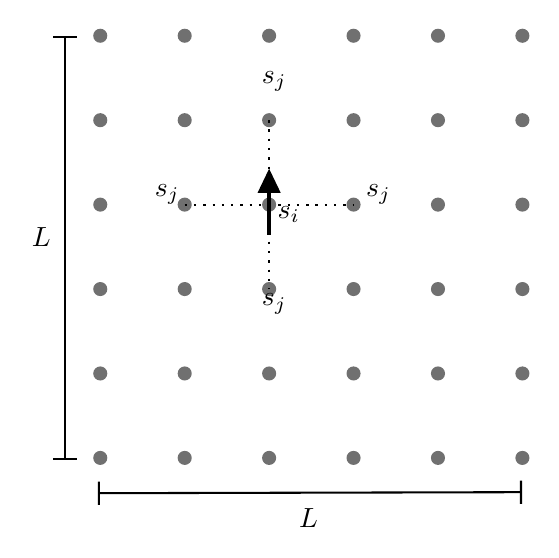
\begin{tikzpicture}[x=0.75pt,y=0.75pt,yscale=-1,xscale=1]
%uncomment if require: \path (0,300); %set diagram left start at 0, and has height of 300

%Shape: Circle [id:dp9447212405494614] 
\draw  [draw opacity=0][fill={rgb, 255:red, 0; green, 0; blue, 0 }  ,fill opacity=0.56 ] (259.83,37.1) .. controls (259.83,35.23) and (261.35,33.71) .. (263.22,33.71) .. controls (265.09,33.71) and (266.61,35.23) .. (266.61,37.1) .. controls (266.61,38.97) and (265.09,40.49) .. (263.22,40.49) .. controls (261.35,40.49) and (259.83,38.97) .. (259.83,37.1) -- cycle ;
%Shape: Circle [id:dp8608297231825602] 
\draw  [draw opacity=0][fill={rgb, 255:red, 0; green, 0; blue, 0 }  ,fill opacity=0.56 ] (300.51,37.1) .. controls (300.51,35.23) and (302.03,33.71) .. (303.9,33.71) .. controls (305.77,33.71) and (307.29,35.23) .. (307.29,37.1) .. controls (307.29,38.97) and (305.77,40.49) .. (303.9,40.49) .. controls (302.03,40.49) and (300.51,38.97) .. (300.51,37.1) -- cycle ;
%Shape: Ellipse [id:dp0047485051715655535] 
\draw  [draw opacity=0][fill={rgb, 255:red, 0; green, 0; blue, 0 }  ,fill opacity=0.56 ] (259.83,77.78) .. controls (259.83,75.91) and (261.35,74.39) .. (263.22,74.39) .. controls (265.09,74.39) and (266.61,75.91) .. (266.61,77.78) .. controls (266.61,79.65) and (265.09,81.17) .. (263.22,81.17) .. controls (261.35,81.17) and (259.83,79.65) .. (259.83,77.78) -- cycle ;
%Shape: Ellipse [id:dp006454201860315978] 
\draw  [draw opacity=0][fill={rgb, 255:red, 0; green, 0; blue, 0 }  ,fill opacity=0.56 ] (300.51,77.78) .. controls (300.51,75.91) and (302.03,74.39) .. (303.9,74.39) .. controls (305.77,74.39) and (307.29,75.91) .. (307.29,77.78) .. controls (307.29,79.65) and (305.77,81.17) .. (303.9,81.17) .. controls (302.03,81.17) and (300.51,79.65) .. (300.51,77.78) -- cycle ;
%Shape: Circle [id:dp6137593483612289] 
\draw  [draw opacity=0][fill={rgb, 255:red, 0; green, 0; blue, 0 }  ,fill opacity=0.56 ] (341.19,37.1) .. controls (341.19,35.23) and (342.7,33.71) .. (344.58,33.71) .. controls (346.45,33.71) and (347.97,35.23) .. (347.97,37.1) .. controls (347.97,38.97) and (346.45,40.49) .. (344.58,40.49) .. controls (342.7,40.49) and (341.19,38.97) .. (341.19,37.1) -- cycle ;
%Shape: Ellipse [id:dp7980079474021842] 
\draw  [draw opacity=0][fill={rgb, 255:red, 0; green, 0; blue, 0 }  ,fill opacity=0.56 ] (381.86,37.1) .. controls (381.86,35.23) and (383.38,33.71) .. (385.25,33.71) .. controls (387.13,33.71) and (388.64,35.23) .. (388.64,37.1) .. controls (388.64,38.97) and (387.13,40.49) .. (385.25,40.49) .. controls (383.38,40.49) and (381.86,38.97) .. (381.86,37.1) -- cycle ;
%Shape: Ellipse [id:dp6932409188666048] 
\draw  [draw opacity=0][fill={rgb, 255:red, 0; green, 0; blue, 0 }  ,fill opacity=0.56 ] (341.19,77.78) .. controls (341.19,75.91) and (342.7,74.39) .. (344.58,74.39) .. controls (346.45,74.39) and (347.97,75.91) .. (347.97,77.78) .. controls (347.97,79.65) and (346.45,81.17) .. (344.58,81.17) .. controls (342.7,81.17) and (341.19,79.65) .. (341.19,77.78) -- cycle ;
%Shape: Ellipse [id:dp014163541337048002] 
\draw  [draw opacity=0][fill={rgb, 255:red, 0; green, 0; blue, 0 }  ,fill opacity=0.56 ] (381.86,77.78) .. controls (381.86,75.91) and (383.38,74.39) .. (385.25,74.39) .. controls (387.13,74.39) and (388.64,75.91) .. (388.64,77.78) .. controls (388.64,79.65) and (387.13,81.17) .. (385.25,81.17) .. controls (383.38,81.17) and (381.86,79.65) .. (381.86,77.78) -- cycle ;
%Shape: Ellipse [id:dp8726239532923227] 
\draw  [draw opacity=0][fill={rgb, 255:red, 0; green, 0; blue, 0 }  ,fill opacity=0.56 ] (259.83,118.46) .. controls (259.83,116.59) and (261.35,115.07) .. (263.22,115.07) .. controls (265.09,115.07) and (266.61,116.59) .. (266.61,118.46) .. controls (266.61,120.33) and (265.09,121.85) .. (263.22,121.85) .. controls (261.35,121.85) and (259.83,120.33) .. (259.83,118.46) -- cycle ;
%Shape: Ellipse [id:dp21404840238689193] 
\draw  [draw opacity=0][fill={rgb, 255:red, 0; green, 0; blue, 0 }  ,fill opacity=0.56 ] (300.51,118.46) .. controls (300.51,116.59) and (302.03,115.07) .. (303.9,115.07) .. controls (305.77,115.07) and (307.29,116.59) .. (307.29,118.46) .. controls (307.29,120.33) and (305.77,121.85) .. (303.9,121.85) .. controls (302.03,121.85) and (300.51,120.33) .. (300.51,118.46) -- cycle ;
%Shape: Circle [id:dp6263910318662165] 
\draw  [draw opacity=0][fill={rgb, 255:red, 0; green, 0; blue, 0 }  ,fill opacity=0.56 ] (259.83,159.14) .. controls (259.83,157.26) and (261.35,155.75) .. (263.22,155.75) .. controls (265.09,155.75) and (266.61,157.26) .. (266.61,159.14) .. controls (266.61,161.01) and (265.09,162.53) .. (263.22,162.53) .. controls (261.35,162.53) and (259.83,161.01) .. (259.83,159.14) -- cycle ;
%Shape: Circle [id:dp5091466549678689] 
\draw  [draw opacity=0][fill={rgb, 255:red, 0; green, 0; blue, 0 }  ,fill opacity=0.56 ] (300.51,159.14) .. controls (300.51,157.26) and (302.03,155.75) .. (303.9,155.75) .. controls (305.77,155.75) and (307.29,157.26) .. (307.29,159.14) .. controls (307.29,161.01) and (305.77,162.53) .. (303.9,162.53) .. controls (302.03,162.53) and (300.51,161.01) .. (300.51,159.14) -- cycle ;
%Shape: Ellipse [id:dp06597451401939625] 
\draw  [draw opacity=0][fill={rgb, 255:red, 0; green, 0; blue, 0 }  ,fill opacity=0.56 ] (341.19,118.46) .. controls (341.19,116.59) and (342.7,115.07) .. (344.58,115.07) .. controls (346.45,115.07) and (347.97,116.59) .. (347.97,118.46) .. controls (347.97,120.33) and (346.45,121.85) .. (344.58,121.85) .. controls (342.7,121.85) and (341.19,120.33) .. (341.19,118.46) -- cycle ;
%Shape: Ellipse [id:dp7659081932907452] 
\draw  [draw opacity=0][fill={rgb, 255:red, 0; green, 0; blue, 0 }  ,fill opacity=0.56 ] (381.86,118.46) .. controls (381.86,116.59) and (383.38,115.07) .. (385.25,115.07) .. controls (387.13,115.07) and (388.64,116.59) .. (388.64,118.46) .. controls (388.64,120.33) and (387.13,121.85) .. (385.25,121.85) .. controls (383.38,121.85) and (381.86,120.33) .. (381.86,118.46) -- cycle ;
%Shape: Circle [id:dp3521970449917553] 
\draw  [draw opacity=0][fill={rgb, 255:red, 0; green, 0; blue, 0 }  ,fill opacity=0.56 ] (341.19,159.14) .. controls (341.19,157.26) and (342.7,155.75) .. (344.58,155.75) .. controls (346.45,155.75) and (347.97,157.26) .. (347.97,159.14) .. controls (347.97,161.01) and (346.45,162.53) .. (344.58,162.53) .. controls (342.7,162.53) and (341.19,161.01) .. (341.19,159.14) -- cycle ;
%Shape: Ellipse [id:dp4307471784456245] 
\draw  [draw opacity=0][fill={rgb, 255:red, 0; green, 0; blue, 0 }  ,fill opacity=0.56 ] (381.86,159.14) .. controls (381.86,157.26) and (383.38,155.75) .. (385.25,155.75) .. controls (387.13,155.75) and (388.64,157.26) .. (388.64,159.14) .. controls (388.64,161.01) and (387.13,162.53) .. (385.25,162.53) .. controls (383.38,162.53) and (381.86,161.01) .. (381.86,159.14) -- cycle ;
%Shape: Circle [id:dp027147569121899973] 
\draw  [draw opacity=0][fill={rgb, 255:red, 0; green, 0; blue, 0 }  ,fill opacity=0.56 ] (422.54,37.1) .. controls (422.54,35.23) and (424.06,33.71) .. (425.93,33.71) .. controls (427.8,33.71) and (429.32,35.23) .. (429.32,37.1) .. controls (429.32,38.97) and (427.8,40.49) .. (425.93,40.49) .. controls (424.06,40.49) and (422.54,38.97) .. (422.54,37.1) -- cycle ;
%Shape: Ellipse [id:dp5740679139072606] 
\draw  [draw opacity=0][fill={rgb, 255:red, 0; green, 0; blue, 0 }  ,fill opacity=0.56 ] (422.54,77.78) .. controls (422.54,75.91) and (424.06,74.39) .. (425.93,74.39) .. controls (427.8,74.39) and (429.32,75.91) .. (429.32,77.78) .. controls (429.32,79.65) and (427.8,81.17) .. (425.93,81.17) .. controls (424.06,81.17) and (422.54,79.65) .. (422.54,77.78) -- cycle ;
%Shape: Ellipse [id:dp3625041731348051] 
\draw  [draw opacity=0][fill={rgb, 255:red, 0; green, 0; blue, 0 }  ,fill opacity=0.56 ] (422.54,118.46) .. controls (422.54,116.59) and (424.06,115.07) .. (425.93,115.07) .. controls (427.8,115.07) and (429.32,116.59) .. (429.32,118.46) .. controls (429.32,120.33) and (427.8,121.85) .. (425.93,121.85) .. controls (424.06,121.85) and (422.54,120.33) .. (422.54,118.46) -- cycle ;
%Shape: Circle [id:dp4989897554599463] 
\draw  [draw opacity=0][fill={rgb, 255:red, 0; green, 0; blue, 0 }  ,fill opacity=0.56 ] (422.54,159.14) .. controls (422.54,157.26) and (424.06,155.75) .. (425.93,155.75) .. controls (427.8,155.75) and (429.32,157.26) .. (429.32,159.14) .. controls (429.32,161.01) and (427.8,162.53) .. (425.93,162.53) .. controls (424.06,162.53) and (422.54,161.01) .. (422.54,159.14) -- cycle ;
%Shape: Circle [id:dp712737118906141] 
\draw  [draw opacity=0][fill={rgb, 255:red, 0; green, 0; blue, 0 }  ,fill opacity=0.56 ] (463.22,37.1) .. controls (463.22,35.23) and (464.74,33.71) .. (466.61,33.71) .. controls (468.48,33.71) and (470,35.23) .. (470,37.1) .. controls (470,38.97) and (468.48,40.49) .. (466.61,40.49) .. controls (464.74,40.49) and (463.22,38.97) .. (463.22,37.1) -- cycle ;
%Shape: Ellipse [id:dp8067942621815305] 
\draw  [draw opacity=0][fill={rgb, 255:red, 0; green, 0; blue, 0 }  ,fill opacity=0.56 ] (463.22,77.78) .. controls (463.22,75.91) and (464.74,74.39) .. (466.61,74.39) .. controls (468.48,74.39) and (470,75.91) .. (470,77.78) .. controls (470,79.65) and (468.48,81.17) .. (466.61,81.17) .. controls (464.74,81.17) and (463.22,79.65) .. (463.22,77.78) -- cycle ;
%Shape: Ellipse [id:dp30470067808885726] 
\draw  [draw opacity=0][fill={rgb, 255:red, 0; green, 0; blue, 0 }  ,fill opacity=0.56 ] (463.22,118.46) .. controls (463.22,116.59) and (464.74,115.07) .. (466.61,115.07) .. controls (468.48,115.07) and (470,116.59) .. (470,118.46) .. controls (470,120.33) and (468.48,121.85) .. (466.61,121.85) .. controls (464.74,121.85) and (463.22,120.33) .. (463.22,118.46) -- cycle ;
%Shape: Circle [id:dp2183382027793922] 
\draw  [draw opacity=0][fill={rgb, 255:red, 0; green, 0; blue, 0 }  ,fill opacity=0.56 ] (463.22,159.14) .. controls (463.22,157.26) and (464.74,155.75) .. (466.61,155.75) .. controls (468.48,155.75) and (470,157.26) .. (470,159.14) .. controls (470,161.01) and (468.48,162.53) .. (466.61,162.53) .. controls (464.74,162.53) and (463.22,161.01) .. (463.22,159.14) -- cycle ;
%Shape: Ellipse [id:dp42413841931764784] 
\draw  [draw opacity=0][fill={rgb, 255:red, 0; green, 0; blue, 0 }  ,fill opacity=0.56 ] (259.83,199.81) .. controls (259.83,197.94) and (261.35,196.42) .. (263.22,196.42) .. controls (265.09,196.42) and (266.61,197.94) .. (266.61,199.81) .. controls (266.61,201.69) and (265.09,203.2) .. (263.22,203.2) .. controls (261.35,203.2) and (259.83,201.69) .. (259.83,199.81) -- cycle ;
%Shape: Ellipse [id:dp7464467165798186] 
\draw  [draw opacity=0][fill={rgb, 255:red, 0; green, 0; blue, 0 }  ,fill opacity=0.56 ] (300.51,199.81) .. controls (300.51,197.94) and (302.03,196.42) .. (303.9,196.42) .. controls (305.77,196.42) and (307.29,197.94) .. (307.29,199.81) .. controls (307.29,201.69) and (305.77,203.2) .. (303.9,203.2) .. controls (302.03,203.2) and (300.51,201.69) .. (300.51,199.81) -- cycle ;
%Shape: Circle [id:dp3742479378652307] 
\draw  [draw opacity=0][fill={rgb, 255:red, 0; green, 0; blue, 0 }  ,fill opacity=0.56 ] (259.83,240.49) .. controls (259.83,238.62) and (261.35,237.1) .. (263.22,237.1) .. controls (265.09,237.1) and (266.61,238.62) .. (266.61,240.49) .. controls (266.61,242.36) and (265.09,243.88) .. (263.22,243.88) .. controls (261.35,243.88) and (259.83,242.36) .. (259.83,240.49) -- cycle ;
%Shape: Circle [id:dp47533976452036275] 
\draw  [draw opacity=0][fill={rgb, 255:red, 0; green, 0; blue, 0 }  ,fill opacity=0.56 ] (300.51,240.49) .. controls (300.51,238.62) and (302.03,237.1) .. (303.9,237.1) .. controls (305.77,237.1) and (307.29,238.62) .. (307.29,240.49) .. controls (307.29,242.36) and (305.77,243.88) .. (303.9,243.88) .. controls (302.03,243.88) and (300.51,242.36) .. (300.51,240.49) -- cycle ;
%Shape: Ellipse [id:dp9074102634030522] 
\draw  [draw opacity=0][fill={rgb, 255:red, 0; green, 0; blue, 0 }  ,fill opacity=0.56 ] (341.19,199.81) .. controls (341.19,197.94) and (342.7,196.42) .. (344.58,196.42) .. controls (346.45,196.42) and (347.97,197.94) .. (347.97,199.81) .. controls (347.97,201.69) and (346.45,203.2) .. (344.58,203.2) .. controls (342.7,203.2) and (341.19,201.69) .. (341.19,199.81) -- cycle ;
%Shape: Ellipse [id:dp34280117941316224] 
\draw  [draw opacity=0][fill={rgb, 255:red, 0; green, 0; blue, 0 }  ,fill opacity=0.56 ] (381.86,199.81) .. controls (381.86,197.94) and (383.38,196.42) .. (385.25,196.42) .. controls (387.13,196.42) and (388.64,197.94) .. (388.64,199.81) .. controls (388.64,201.69) and (387.13,203.2) .. (385.25,203.2) .. controls (383.38,203.2) and (381.86,201.69) .. (381.86,199.81) -- cycle ;
%Shape: Circle [id:dp4297673435931586] 
\draw  [draw opacity=0][fill={rgb, 255:red, 0; green, 0; blue, 0 }  ,fill opacity=0.56 ] (341.19,240.49) .. controls (341.19,238.62) and (342.7,237.1) .. (344.58,237.1) .. controls (346.45,237.1) and (347.97,238.62) .. (347.97,240.49) .. controls (347.97,242.36) and (346.45,243.88) .. (344.58,243.88) .. controls (342.7,243.88) and (341.19,242.36) .. (341.19,240.49) -- cycle ;
%Shape: Ellipse [id:dp4933319042062405] 
\draw  [draw opacity=0][fill={rgb, 255:red, 0; green, 0; blue, 0 }  ,fill opacity=0.56 ] (381.86,240.49) .. controls (381.86,238.62) and (383.38,237.1) .. (385.25,237.1) .. controls (387.13,237.1) and (388.64,238.62) .. (388.64,240.49) .. controls (388.64,242.36) and (387.13,243.88) .. (385.25,243.88) .. controls (383.38,243.88) and (381.86,242.36) .. (381.86,240.49) -- cycle ;
%Shape: Ellipse [id:dp2777034075992263] 
\draw  [draw opacity=0][fill={rgb, 255:red, 0; green, 0; blue, 0 }  ,fill opacity=0.56 ] (422.54,199.81) .. controls (422.54,197.94) and (424.06,196.42) .. (425.93,196.42) .. controls (427.8,196.42) and (429.32,197.94) .. (429.32,199.81) .. controls (429.32,201.69) and (427.8,203.2) .. (425.93,203.2) .. controls (424.06,203.2) and (422.54,201.69) .. (422.54,199.81) -- cycle ;
%Shape: Circle [id:dp7756258257121033] 
\draw  [draw opacity=0][fill={rgb, 255:red, 0; green, 0; blue, 0 }  ,fill opacity=0.56 ] (422.54,240.49) .. controls (422.54,238.62) and (424.06,237.1) .. (425.93,237.1) .. controls (427.8,237.1) and (429.32,238.62) .. (429.32,240.49) .. controls (429.32,242.36) and (427.8,243.88) .. (425.93,243.88) .. controls (424.06,243.88) and (422.54,242.36) .. (422.54,240.49) -- cycle ;
%Shape: Ellipse [id:dp45143449643890765] 
\draw  [draw opacity=0][fill={rgb, 255:red, 0; green, 0; blue, 0 }  ,fill opacity=0.56 ] (463.22,199.81) .. controls (463.22,197.94) and (464.74,196.42) .. (466.61,196.42) .. controls (468.48,196.42) and (470,197.94) .. (470,199.81) .. controls (470,201.69) and (468.48,203.2) .. (466.61,203.2) .. controls (464.74,203.2) and (463.22,201.69) .. (463.22,199.81) -- cycle ;
%Shape: Circle [id:dp679521683918024] 
\draw  [draw opacity=0][fill={rgb, 255:red, 0; green, 0; blue, 0 }  ,fill opacity=0.56 ] (463.22,240.49) .. controls (463.22,238.62) and (464.74,237.1) .. (466.61,237.1) .. controls (468.48,237.1) and (470,238.62) .. (470,240.49) .. controls (470,242.36) and (468.48,243.88) .. (466.61,243.88) .. controls (464.74,243.88) and (463.22,242.36) .. (463.22,240.49) -- cycle ;
%Straight Lines [id:da07940753860654459] 
\draw [line width=1.5]    (344.58,133.03) -- (344.58,128.97) -- (344.58,105.17) ;
\draw [shift={(344.58,101.17)}, rotate = 90] [fill={rgb, 255:red, 0; green, 0; blue, 0 }  ][line width=0.08]  [draw opacity=0] (11.61,-5.58) -- (0,0) -- (11.61,5.58) -- cycle    ;
%Straight Lines [id:da4557006627729121] 
\draw  [dash pattern={on 0.84pt off 2.51pt}]  (303.9,118.46) -- (344.58,118.46) ;
%Straight Lines [id:da6011978221286447] 
\draw  [dash pattern={on 0.84pt off 2.51pt}]  (344.58,118.46) -- (385.25,118.46) ;
%Straight Lines [id:da8595948878716739] 
\draw  [dash pattern={on 0.84pt off 2.51pt}]  (344.58,118.46) -- (344.58,159.14) ;
%Straight Lines [id:da11277063416864641] 
\draw  [dash pattern={on 0.84pt off 2.51pt}]  (344.58,77.78) -- (344.58,118.46) ;
%Straight Lines [id:da696695291664677] 
\draw    (246.27,37.78) -- (246.27,62.19) -- (246.27,241.17) ;
\draw [shift={(246.27,241.17)}, rotate = 270] [color={rgb, 255:red, 0; green, 0; blue, 0 }  ][line width=0.75]    (0,5.59) -- (0,-5.59)   ;
\draw [shift={(246.27,37.78)}, rotate = 270] [color={rgb, 255:red, 0; green, 0; blue, 0 }  ][line width=0.75]    (0,5.59) -- (0,-5.59)   ;
%Straight Lines [id:da4794241811303237] 
\draw    (262.54,257.5) -- (286.95,257.44) -- (465.93,257) ;
\draw [shift={(465.93,257)}, rotate = 179.86] [color={rgb, 255:red, 0; green, 0; blue, 0 }  ][line width=0.75]    (0,5.59) -- (0,-5.59)   ;
\draw [shift={(262.54,257.5)}, rotate = 179.86] [color={rgb, 255:red, 0; green, 0; blue, 0 }  ][line width=0.75]    (0,5.59) -- (0,-5.59)   ;

% Text Node
\draw (347.23,117.99) node [anchor=north west][inner sep=0.75pt]    {$s_{i}$};
% Text Node
\draw (228.75,127.81) node [anchor=north west][inner sep=0.75pt]    {$L$};
% Text Node
\draw (357.56,263.4) node [anchor=north west][inner sep=0.75pt]    {$L$};
% Text Node
\draw (339.61,52.91) node [anchor=north west][inner sep=0.75pt]    {$s_{j}$};
% Text Node
\draw (389.78,107.15) node [anchor=north west][inner sep=0.75pt]    {$s_{j}$};
% Text Node
\draw (288.08,107.15) node [anchor=north west][inner sep=0.75pt]    {$s_{j}$};
% Text Node
\draw (339.61,160.03) node [anchor=north west][inner sep=0.75pt]    {$s_{j}$};


\end{tikzpicture}

    \caption{A spin $s_i$ on the lattice and its nearest neighbours $s_j$}
\end{figure}

The Hamiltonian is defined to be

$$
    H = -J \sum_{\langle i,j \rangle}s_i s_j -G\sum_i s_i
$$

where the sum $\langle i j \rangle$ is over nearest neighbours as shown in the above diagram. $J$ represents the coupling strength between individual spins while $G$ represents the interaction of the spins with a honmogenous external magnetic field. Observables of interest are the total energy $E$, total magnetization $M$, as well as the magnetic susceptibility $\chi$ and heat capacity $C_V$:

\begin{align*}
    \chi    &= \langle M^2 \rangle - \langle M \rangle^2 \\
    C_V     &= \langle E^2 \rangle - \langle E \rangle^2
\end{align*}    

As the system is liable to exhibit thermal fluctuations, we must calculate ensemble averages of the above observables. However owing to the large ($2^{L^2}$) number of configurations, this is not viable. Hence we resort to Monte Carlo techniques, sampling possible configurations in order to calculate the averages.

As the system is in equilibrium with a heat-bath we expect the configurations to follow Boltzman statistics. We use the Metropolis method to generate a finite of configurations that are representative of the entire phase space, thus yielding the correct ensemble averages. This is done using Markov chains.

The master equation for a Markov process is

$$
    \rho(X,t+1) - \rho(X,t) = - \sum_{X^\prime} T(X\rightarrow X^\prime)\rho(X,t) + \sum_{X^\prime} T(X^\prime \rightarrow X)\rho(X^\prime,t)
$$

We are interested in the stationary distribution $\rho(X)$ for which the left side vanishes. One possible solution is the detailed balance condition where in the long run the rates of both opposing processes become equal:
$$
    \frac{T(X\rightarrow X^\prime)}{T(X^\prime \rightarrow X)} = \frac{\rho(X,t)}{\rho(X^\prime,t)}
$$

We the write the transition probabilities in the form

$$
    T(X \rightarrow X^\prime) = A_{X X^\prime} \omega_{X X^\prime}
$$

where $ 0\leq \omega_{X X^\prime} \leq 1$, $\sum_{X}\sum_{X^\prime} \omega_{X X^\prime} = 1$, and $\omega_{X X^\prime} = \omega_{X^\prime X}$

We then have 

$$
    \frac{A_{X X^\prime}}{A_{X^\prime X}} = \frac{\rho (X^\prime)}{\rho(X)}
$$

Our targetted stationary distribution is the Boltzmann distribution, so

\begin{align*}
\frac{\rho(X^\prime)}{\rho(X)} &= e^{-\beta(H[X^\prime] - H[X])} = e^{-\beta \Delta H}\\
\implies \frac{A_{X X^\prime}}{A_{X^\prime X}} &= e^{-\beta \Delta H}
\end{align*}


\newpage

\header{Flowchart:}

% \begin{figure}[!htb]
%     \centering
%     \begin{tikzpicture}[node distance=2cm]
%         \node (start) [startstop] {Start};
%     \end{tikzpicture}
% \end{figure}

\newpage

\small\texttt{\verbatiminput{code/7_ising.f90}}

\newpage

\header{Output:}

\begin{figure*}[!htb]
    \centering
    \includegraphics[width=1.0\linewidth]{diag/ising_mag.png}
    \caption{Magnetization per spin}
    \label{fig:placeholder}
\end{figure*}

\begin{figure*}[!htb]
    \centering
    \includegraphics[width=1.0\linewidth]{diag/ising_energy.png}
    \caption{Energy per spin}
    \label{fig:placeholder}
\end{figure*}

\begin{figure*}[!htb]
    \centering
    \includegraphics[width=1.0\linewidth]{diag/ising_heatcap.png}
    \caption{Heat Capacity per spin}
    \label{fig:placeholder}
\end{figure*}

\begin{figure*}[!htb]
    \centering
    \includegraphics[width=1.0\linewidth]{diag/ising_susc.png}
    \caption{Magnetic Susceptibility per spin}
    \label{fig:placeholder}
\end{figure*}

\vspace{2em}
